%% Chapter 8: Linearization
%% IEEE-format Control Systems Textbook
%% Self-contained chapter on nonlinear to linear approximation

\chapter{Linearization}
\label{ch:linearization}

\begin{quote}
\textit{``The whole of mathematics consists in the organization of a series of aids to the imagination in the process of reasoning.''} --- Alfred North Whitehead
\end{quote}

\section{Historical Motivation: From Newton to Modern Control}

The story of linearization is, in many ways, the story of applied mathematics itself. It represents humanity's pragmatic response to a fundamental truth: most physical systems are inherently nonlinear, yet our mathematical tools for analyzing nonlinear systems remain severely limited. Linearization is the bridge that allows us to apply the powerful machinery of linear algebra and differential equations to the messy reality of physical systems.

\subsection{Newton and the Birth of Local Approximation (1687)}

\begin{historicalbox}[Newton's Revolutionary Insight]
Isaac Newton's \textit{Principia Mathematica}, published in 1687, laid the foundation for both calculus and the concept of local approximation. Newton recognized that complicated functions could be represented as infinite series---what we now call Taylor series or power series expansions. In his \textit{Method of Fluxions}, Newton developed techniques for expanding functions around a point:
\begin{equation}
f(x) = f(x_0) + f'(x_0)(x - x_0) + \frac{f''(x_0)}{2!}(x - x_0)^2 + \cdots
\end{equation}

The revolutionary insight was that \textit{near} the expansion point $x_0$, the higher-order terms become negligibly small. If $(x - x_0)$ is small, then $(x - x_0)^2$ is smaller still, and $(x - x_0)^3$ even more so. This observation---that locally, any smooth function can be approximated by a straight line---is the mathematical foundation of linearization.

Newton himself applied this principle in his analysis of planetary motion. While the gravitational interactions of multiple bodies create hopelessly complex nonlinear dynamics, Newton showed that for small perturbations from a known orbit, the motion could be approximated by linear equations. This ``perturbation theory'' became a cornerstone of celestial mechanics.
\end{historicalbox}

\subsection{Small Oscillation Theory in Physics}

The 18th and 19th centuries saw the systematic application of linearization to problems in physics, particularly in the study of oscillations. Consider the simple pendulum, whose exact equation of motion is:
\begin{equation}
\ddot{\theta} + \frac{g}{L}\sin(\theta) = 0
\end{equation}

This equation has no closed-form solution in terms of elementary functions. However, physicists from Huygens onward recognized that for small angles, $\sin(\theta) \approx \theta$, yielding:
\begin{equation}
\ddot{\theta} + \frac{g}{L}\theta = 0
\end{equation}

This is the equation of simple harmonic motion, with the well-known solution $\theta(t) = A\cos(\omega_n t + \phi)$ where $\omega_n = \sqrt{g/L}$. The period $T = 2\pi\sqrt{L/g}$ is independent of amplitude---but only in the linear approximation.

Joseph-Louis Lagrange (1736--1813) systematized this approach in his \textit{M\'{e}canique Analytique} (1788), developing a general theory of small oscillations for systems with multiple degrees of freedom. His method proceeded by first finding the equilibrium configuration, then expanding the potential and kinetic energies to second order about that equilibrium. From these quadratic approximations, he derived linearized equations of motion, which could then be solved to find the ``normal modes'' of oscillation---the natural patterns in which the system vibrates. This framework remains the standard approach for vibration analysis in mechanical engineering.

\subsection{Poincar\'{e} and the Qualitative Theory (1880s)}

Henri Poincar\'{e} (1854--1912) revolutionized the study of differential equations by shifting focus from exact solutions to qualitative behavior. In his work on the three-body problem and celestial mechanics, Poincar\'{e} recognized that understanding the geometry of solutions---their stability, periodic orbits, and long-term behavior---was more valuable than explicit formulas.

Poincar\'{e}'s key contribution to linearization was the concept of \textbf{local stability analysis}. He showed that the stability of an equilibrium point of a nonlinear system:
\begin{equation}
\dot{x} = f(x)
\end{equation}
could be determined by examining the linearized system:
\begin{equation}
\delta\dot{x} = \frac{\partial f}{\partial x}\bigg|_{x_0} \delta x
\end{equation}

If all eigenvalues of the Jacobian matrix $\partial f/\partial x|_{x_0}$ have negative real parts, the equilibrium is locally asymptotically stable. This principle, formalized by Lyapunov shortly after, remains the primary tool for stability analysis in control theory.

Poincar\'{e} also introduced the concept of the \textbf{phase portrait}---a graphical representation of system trajectories in state space. The phase portrait of a nonlinear system near an equilibrium point closely resembles that of its linearization, provided the eigenvalues have non-zero real parts (hyperbolic equilibria). This observation justifies the use of linear analysis for local behavior.

\subsection{Aircraft Stability Analysis (1900s)}

The development of powered flight created an urgent need for stability analysis of complex dynamic systems. The Wright Brothers' 1903 Flyer was deliberately designed to be unstable, requiring constant pilot input---a choice that gave them better control authority but made flight exhausting and dangerous.

By the 1910s, aviation pioneers recognized that stable aircraft were essential for practical flight. Frederick Lanchester in England and George Bryan in the United States developed the mathematical framework for aircraft stability, based entirely on linearization.

An aircraft in flight obeys nonlinear equations of motion with six degrees of freedom (three translations, three rotations). The full equations involve trigonometric functions, aerodynamic forces that depend on angle of attack in complicated ways, and coupling between all axes. Exact analysis is intractable.

The breakthrough was the concept of the \textbf{trim condition}: a steady, level flight condition where all forces and moments balance. Small perturbations from trim satisfy linearized equations:
\begin{equation}
\begin{bmatrix} \delta\dot{u} \\ \delta\dot{w} \\ \delta\dot{q} \\ \delta\dot{\theta} \end{bmatrix} =
\begin{bmatrix} X_u & X_w & X_q & -g\cos\theta_0 \\
Z_u & Z_w & Z_q & -g\sin\theta_0 \\
M_u & M_w & M_q & 0 \\
0 & 0 & 1 & 0 \end{bmatrix}
\begin{bmatrix} \delta u \\ \delta w \\ \delta q \\ \delta\theta \end{bmatrix}
\end{equation}

Here $\delta u, \delta w$ are perturbations in forward and vertical velocity, $\delta q$ is pitch rate perturbation, and $\delta\theta$ is pitch angle perturbation. The ``stability derivatives'' $X_u, Z_w, M_q$, etc., are partial derivatives of aerodynamic forces and moments with respect to state variables, evaluated at trim.

This linearized model enabled engineers to predict natural frequencies such as the phugoid and short period modes, design control surfaces with adequate stability margins, analyze pilot-in-the-loop handling qualities, and develop autopilot systems. The success of linearized aircraft dynamics established the paradigm that dominates control engineering: \textit{design around an operating point}.

\subsection{Why Linearize? The Practical Argument}

Nonlinear differential equations are \textbf{hard}. The principle of superposition, which states that for linear systems any combination $\alpha x_1(t) + \beta x_2(t)$ of solutions is also a solution, does not hold for nonlinear systems. This superposition principle is what allows us to analyze complex inputs by decomposing them into simpler components through Fourier analysis and convolution. Furthermore, while linear differential equations with constant coefficients can always be solved using eigenvalue methods, most nonlinear equations have no closed-form solutions. The Laplace transform, which converts linear ODEs to algebraic equations and enables frequency-domain analysis, is not applicable to nonlinear systems. Finally, stability analysis becomes far more complex: for linear systems, stability depends only on eigenvalue locations, whereas nonlinear systems can exhibit limit cycles, chaos, and other behaviors that linear theory cannot predict.

Linear systems, by contrast, are mathematically tractable. They admit complete solutions via eigenvalue decomposition and can be represented by transfer functions that enable frequency response analysis. Classical design methods such as root locus and Bode plots become available, along with modern techniques including state feedback and observer design via pole placement. Optimal control approaches, particularly Linear-Quadratic Regulator (LQR) design and Kalman filtering, round out the powerful toolkit available for linear systems.

The entire toolkit of classical and modern control theory---Chapters 9--20 of this textbook---assumes linear system models. Linearization is the gateway that allows us to apply these powerful methods to real, nonlinear systems.

\textbf{The engineering assumption:} Most control systems are designed to keep the system near a desired operating point. A thermostat maintains room temperature near a setpoint; an autopilot holds altitude and heading near desired values; a robot arm tracks a smooth trajectory. If the controller works properly, perturbations from the operating point remain small, and the linear approximation is valid.

This is a self-fulfilling prophecy: we design controllers using linear theory, and those controllers (when successful) keep the system in the region where linear theory is valid.

%% ============================================================================
\section{Modern Applications of Linearization}
\label{sec:linearization_applications}

Linearization is not merely a historical curiosity; it remains the dominant approach for control system design across virtually every engineering domain. This section surveys modern applications where linearization enables sophisticated control of inherently nonlinear systems.

\subsection{Aircraft Autopilot Design}

Modern commercial aircraft operate with sophisticated autopilot systems that control altitude, heading, speed, and approach trajectories. Despite the nonlinear nature of aircraft dynamics, these systems are designed entirely using linearized models.

The process begins with a detailed nonlinear simulation model that captures aerodynamic forces as functions of angle of attack, sideslip, and Mach number, along with engine thrust characteristics across the flight envelope. The model also incorporates atmospheric variations with altitude and actuator dynamics including rate limits.

At each flight condition (altitude, airspeed, weight), the nonlinear model is linearized to produce state-space matrices $(A, B, C, D)$. Control laws are designed for each linearization point, and gain scheduling interpolates between designs as flight conditions change.

This approach has proven remarkably successful. The Boeing 777, for example, uses a fly-by-wire system with linearization-based control laws that safely operate across the entire flight envelope---from takeoff to landing, in turbulence and wind shear, with engine failures and other contingencies.

\subsection{Chemical Process Control}

Chemical reactors exhibit strongly nonlinear behavior arising from several sources. The Arrhenius temperature dependence of reaction rates, expressed as $k = A e^{-E_a/RT}$, introduces exponential nonlinearity. Heat transfer is inherently nonlinear, especially when phase changes occur. Reaction kinetics depend on concentrations in complex ways, and many reactors exhibit multiple steady states with the potential for thermal runaway.

Despite this complexity, most industrial process control uses PID controllers designed via linearization. At the desired operating point (setpoint), the process is linearized to determine appropriate controller gains. Advanced regulatory control uses model predictive control (MPC) with linearized models updated in real-time.

The key insight is that a well-designed control system prevents the large deviations that would make linearization invalid. Temperature excursions, concentration swings, and pressure variations are kept small by feedback control---exactly the regime where linear models are accurate.

\subsection{Power Electronics: Small-Signal Analysis}

Switch-mode power supplies, motor drives, and renewable energy inverters involve switching nonlinearities that seem to defy linear analysis. However, the concept of ``small-signal analysis'' applies linearization to these systems with remarkable success.

Consider a DC-DC buck converter. The switches (transistors, diodes) are inherently nonlinear. However, if we average the switching behavior over one switching period, we obtain a continuous (but still nonlinear) model. Linearizing around the operating point yields a small-signal model:
\begin{equation}
\hat{v}_o(s) = G_{vd}(s)\hat{d}(s) + G_{vg}(s)\hat{v}_g(s)
\end{equation}
where $\hat{v}_o$ is output voltage perturbation, $\hat{d}$ is duty cycle perturbation, and $\hat{v}_g$ is input voltage perturbation.

This transfer function model enables loop gain analysis for stability assessment, compensator design using Bode plot techniques, input and output impedance calculations, and prediction of transient response characteristics. The entire field of power electronics control is built on this small-signal linearization framework.

\subsection{Robot Arm Control: Jacobian Linearization}

Robot manipulators are highly nonlinear systems. The relationship between joint angles and end-effector position involves trigonometric functions (kinematics), and the dynamics include configuration-dependent inertias, Coriolis forces, and gravity terms.

For trajectory tracking, robots use a combination of feedforward (computed torque) and feedback control. The feedback component typically uses linearization:
\begin{equation}
\delta\dot{x} = J(q)\delta\dot{q}
\end{equation}
where $J(q)$ is the Jacobian matrix relating joint velocities to end-effector velocities.

Near the desired trajectory, the linearized dynamics enable resolved-motion rate control, Cartesian impedance control, and force/position hybrid control schemes. Modern industrial robots achieve submillimeter accuracy by using linearization-based control, with the nonlinear terms handled by feedforward compensation.

%% ============================================================================
\section{Mathematical Foundation}
\label{sec:linearization_math}

This section provides the complete mathematical framework for linearization of nonlinear systems. We begin with a review of Taylor series and progress to the general procedure for multi-input, multi-output systems.

\subsection{Taylor Series Review}

The foundation of linearization is the Taylor series expansion of a smooth function. For a scalar function $f(x)$ of a single variable, expanded about $x_0$:
\begin{equation}
f(x) = f(x_0) + f'(x_0)(x - x_0) + \frac{f''(x_0)}{2!}(x - x_0)^2 + \frac{f'''(x_0)}{3!}(x - x_0)^3 + \cdots
\label{eq:taylor_scalar}
\end{equation}

For small deviations $\delta x = x - x_0$, the higher-order terms become negligible:
\begin{equation}
f(x) \approx f(x_0) + f'(x_0)\delta x + O(\delta x^2)
\end{equation}

The notation $O(\delta x^2)$ indicates terms that scale with the square (or higher powers) of $\delta x$. When $|\delta x| \ll 1$, these terms can be neglected.

For functions of multiple variables, $f(x_1, x_2, \ldots, x_n)$, the Taylor expansion becomes:
\begin{equation}
f(\mathbf{x}) = f(\mathbf{x}_0) + \sum_{i=1}^{n} \frac{\partial f}{\partial x_i}\bigg|_{\mathbf{x}_0} (x_i - x_{0,i}) + \text{higher order terms}
\end{equation}

In vector notation:
\begin{equation}
f(\mathbf{x}) \approx f(\mathbf{x}_0) + \nabla f|_{\mathbf{x}_0}^T (\mathbf{x} - \mathbf{x}_0)
\end{equation}

where $\nabla f$ is the gradient vector.

\begin{figure}[htbp]
\centering
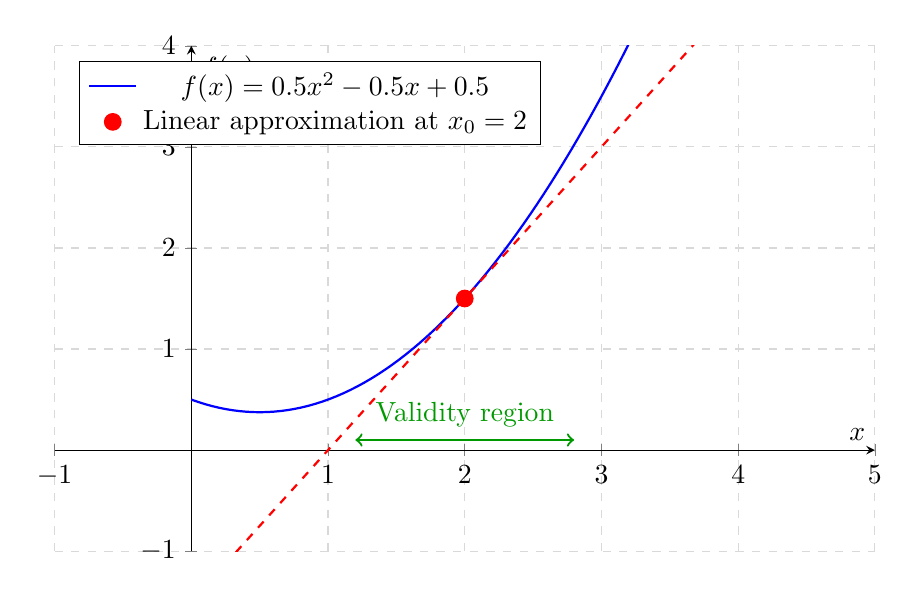
\begin{tikzpicture}
    \begin{axis}[
        width=12cm, height=8cm,
        xlabel={$x$},
        ylabel={$f(x)$},
        xmin=-1, xmax=5,
        ymin=-1, ymax=4,
        axis lines=middle,
        legend pos=north west,
        grid=major,
        grid style={dashed, gray!30}
    ]
    % Nonlinear function
    \addplot[blue, thick, domain=0:5, samples=100] {0.5*x^2 - 0.5*x + 0.5};
    \addlegendentry{$f(x) = 0.5x^2 - 0.5x + 0.5$}

    % Operating point
    \addplot[only marks, mark=*, mark size=3pt, red] coordinates {(2, 1.5)};

    % Tangent line (linearization)
    \addplot[red, thick, dashed, domain=0:4] {1.5 + 1.5*(x-2)};
    \addlegendentry{Linear approximation at $x_0=2$}

    % Validity region
    \draw[<->, thick, green!60!black] (axis cs:1.2,0.1) -- (axis cs:2.8,0.1);
    \node[green!60!black] at (axis cs:2,0.35) {Validity region};

    \end{axis}
\end{tikzpicture}
\caption{Graphical interpretation of linearization. The tangent line (dashed) approximates the nonlinear function (solid) near the operating point $x_0 = 2$. The approximation is accurate within the validity region.}
\label{fig:graphical_linearization}
\end{figure}

\subsection{The Linearization Procedure}

Consider a general nonlinear system described by:
\begin{equation}
\dot{\mathbf{x}} = \mathbf{f}(\mathbf{x}, \mathbf{u})
\label{eq:nonlinear_system}
\end{equation}
where $\mathbf{x} \in \mathbb{R}^n$ is the state vector, $\mathbf{u} \in \mathbb{R}^m$ is the input vector, and $\mathbf{f}: \mathbb{R}^n \times \mathbb{R}^m \rightarrow \mathbb{R}^n$ is a smooth (continuously differentiable) function.

\textbf{Step 1: Find the Equilibrium Point}

An equilibrium (operating) point $(\mathbf{x}_0, \mathbf{u}_0)$ satisfies:
\begin{equation}
\mathbf{f}(\mathbf{x}_0, \mathbf{u}_0) = \mathbf{0}
\label{eq:equilibrium}
\end{equation}

At equilibrium, the state derivative is zero, so the system remains at $\mathbf{x}_0$ when input is held at $\mathbf{u}_0$. For many systems, multiple equilibrium points may exist, and the choice of operating point depends on the desired system behavior.

\textbf{Step 2: Define Perturbation Variables}

Define deviations from the operating point:
\begin{align}
\delta\mathbf{x} &= \mathbf{x} - \mathbf{x}_0 \label{eq:delta_x} \\
\delta\mathbf{u} &= \mathbf{u} - \mathbf{u}_0 \label{eq:delta_u}
\end{align}

\textbf{Step 3: Apply Taylor Series Expansion}

Expand $\mathbf{f}(\mathbf{x}, \mathbf{u})$ about the operating point:
\begin{equation}
\mathbf{f}(\mathbf{x}, \mathbf{u}) = \mathbf{f}(\mathbf{x}_0, \mathbf{u}_0) + \frac{\partial \mathbf{f}}{\partial \mathbf{x}}\bigg|_0 (\mathbf{x} - \mathbf{x}_0) + \frac{\partial \mathbf{f}}{\partial \mathbf{u}}\bigg|_0 (\mathbf{u} - \mathbf{u}_0) + \text{H.O.T.}
\end{equation}

Since $\mathbf{f}(\mathbf{x}_0, \mathbf{u}_0) = \mathbf{0}$ at equilibrium, and noting that $\dot{\mathbf{x}} = \delta\dot{\mathbf{x}}$ (since $\mathbf{x}_0$ is constant):
\begin{equation}
\delta\dot{\mathbf{x}} \approx \frac{\partial \mathbf{f}}{\partial \mathbf{x}}\bigg|_0 \delta\mathbf{x} + \frac{\partial \mathbf{f}}{\partial \mathbf{u}}\bigg|_0 \delta\mathbf{u}
\end{equation}

\textbf{Step 4: Define Jacobian Matrices}

The \textbf{system matrix} (or \textbf{state Jacobian}) is:
\begin{equation}
\mathbf{A} = \frac{\partial \mathbf{f}}{\partial \mathbf{x}}\bigg|_{(\mathbf{x}_0, \mathbf{u}_0)} =
\begin{bmatrix}
\frac{\partial f_1}{\partial x_1} & \frac{\partial f_1}{\partial x_2} & \cdots & \frac{\partial f_1}{\partial x_n} \\
\frac{\partial f_2}{\partial x_1} & \frac{\partial f_2}{\partial x_2} & \cdots & \frac{\partial f_2}{\partial x_n} \\
\vdots & \vdots & \ddots & \vdots \\
\frac{\partial f_n}{\partial x_1} & \frac{\partial f_n}{\partial x_2} & \cdots & \frac{\partial f_n}{\partial x_n}
\end{bmatrix}_{(\mathbf{x}_0, \mathbf{u}_0)}
\label{eq:A_matrix}
\end{equation}

The \textbf{input matrix} (or \textbf{control Jacobian}) is:
\begin{equation}
\mathbf{B} = \frac{\partial \mathbf{f}}{\partial \mathbf{u}}\bigg|_{(\mathbf{x}_0, \mathbf{u}_0)} =
\begin{bmatrix}
\frac{\partial f_1}{\partial u_1} & \frac{\partial f_1}{\partial u_2} & \cdots & \frac{\partial f_1}{\partial u_m} \\
\frac{\partial f_2}{\partial u_1} & \frac{\partial f_2}{\partial u_2} & \cdots & \frac{\partial f_2}{\partial u_m} \\
\vdots & \vdots & \ddots & \vdots \\
\frac{\partial f_n}{\partial u_1} & \frac{\partial f_n}{\partial u_2} & \cdots & \frac{\partial f_n}{\partial u_m}
\end{bmatrix}_{(\mathbf{x}_0, \mathbf{u}_0)}
\label{eq:B_matrix}
\end{equation}

\textbf{Step 5: Write the Linearized Model}

The linearized state-space model is:
\begin{equation}
\boxed{\delta\dot{\mathbf{x}} = \mathbf{A}\delta\mathbf{x} + \mathbf{B}\delta\mathbf{u}}
\label{eq:linearized_model}
\end{equation}

This is a linear, time-invariant (LTI) system in the perturbation variables. All the tools of linear control theory can now be applied.

If there is also an output equation $\mathbf{y} = \mathbf{g}(\mathbf{x}, \mathbf{u})$, it can be linearized similarly:
\begin{equation}
\delta\mathbf{y} = \mathbf{C}\delta\mathbf{x} + \mathbf{D}\delta\mathbf{u}
\end{equation}
where:
\begin{equation}
\mathbf{C} = \frac{\partial \mathbf{g}}{\partial \mathbf{x}}\bigg|_0, \quad \mathbf{D} = \frac{\partial \mathbf{g}}{\partial \mathbf{u}}\bigg|_0
\end{equation}

\subsection{Example: The Simple Pendulum}

The simple pendulum provides an ideal case study for linearization. Consider a pendulum of length $L$ with a point mass $m$, swinging under gravity.

\textbf{Nonlinear Equation of Motion}

From Newton's second law (or Lagrangian mechanics):
\begin{equation}
mL^2\ddot{\theta} = -mgL\sin(\theta)
\end{equation}

Simplifying:
\begin{equation}
\ddot{\theta} + \frac{g}{L}\sin(\theta) = 0
\label{eq:pendulum_nonlinear}
\end{equation}

\textbf{State-Space Formulation}

Define state variables:
\begin{equation}
x_1 = \theta, \quad x_2 = \dot{\theta}
\end{equation}

The state equations are:
\begin{align}
\dot{x}_1 &= x_2 \\
\dot{x}_2 &= -\frac{g}{L}\sin(x_1)
\end{align}

Or in vector form:
\begin{equation}
\dot{\mathbf{x}} = \mathbf{f}(\mathbf{x}) = \begin{bmatrix} x_2 \\ -\frac{g}{L}\sin(x_1) \end{bmatrix}
\end{equation}

\textbf{Equilibrium Points}

Setting $\mathbf{f}(\mathbf{x}) = \mathbf{0}$:
\begin{align}
x_2 &= 0 \\
-\frac{g}{L}\sin(x_1) &= 0
\end{align}

This gives $x_1 = n\pi$ for any integer $n$. The physically meaningful equilibria are $\theta = 0$ (hanging down), which is a stable equilibrium, and $\theta = \pi$ (inverted), which is an unstable equilibrium.

\textbf{Linearization about $\theta = 0$}

At the operating point $\mathbf{x}_0 = [0, 0]^T$:
\begin{equation}
\mathbf{A} = \frac{\partial \mathbf{f}}{\partial \mathbf{x}}\bigg|_0 = \begin{bmatrix} \frac{\partial f_1}{\partial x_1} & \frac{\partial f_1}{\partial x_2} \\ \frac{\partial f_2}{\partial x_1} & \frac{\partial f_2}{\partial x_2} \end{bmatrix}_0 = \begin{bmatrix} 0 & 1 \\ -\frac{g}{L}\cos(x_1) & 0 \end{bmatrix}_{x_1=0} = \begin{bmatrix} 0 & 1 \\ -\frac{g}{L} & 0 \end{bmatrix}
\end{equation}

The linearized system is:
\begin{equation}
\begin{bmatrix} \delta\dot{x}_1 \\ \delta\dot{x}_2 \end{bmatrix} = \begin{bmatrix} 0 & 1 \\ -\frac{g}{L} & 0 \end{bmatrix} \begin{bmatrix} \delta x_1 \\ \delta x_2 \end{bmatrix}
\end{equation}

Converting back to scalar form:
\begin{equation}
\ddot{\theta} + \frac{g}{L}\theta = 0
\label{eq:pendulum_linearized}
\end{equation}

This is simple harmonic motion with natural frequency $\omega_n = \sqrt{g/L}$ and period:
\begin{equation}
T_{\text{linear}} = 2\pi\sqrt{\frac{L}{g}}
\label{eq:linear_period}
\end{equation}

\begin{figure}[htbp]
\centering
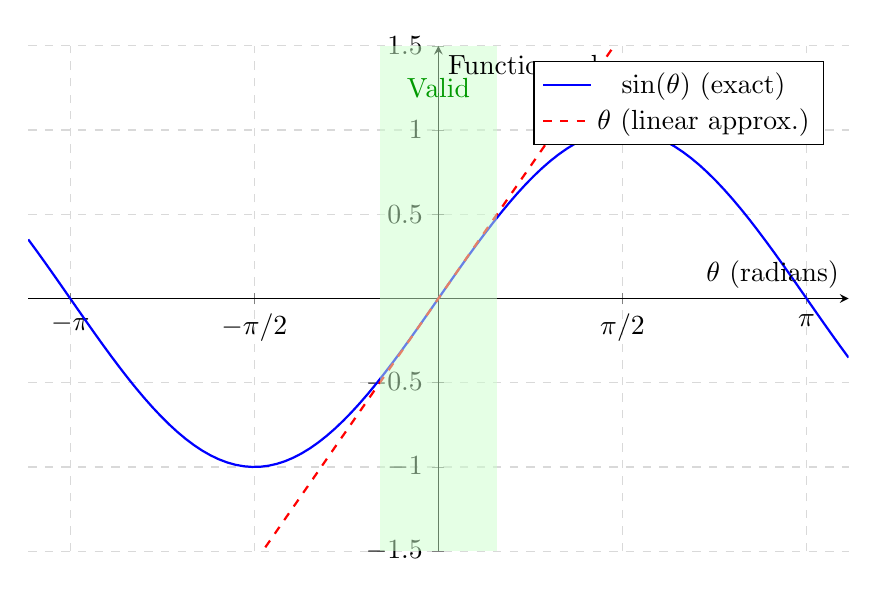
\begin{tikzpicture}
    \begin{axis}[
        width=12cm, height=8cm,
        xlabel={$\theta$ (radians)},
        ylabel={Function value},
        xmin=-3.5, xmax=3.5,
        ymin=-1.5, ymax=1.5,
        axis lines=middle,
        legend pos=north east,
        grid=major,
        grid style={dashed, gray!30},
        xtick={-3.14159, -1.5708, 0, 1.5708, 3.14159},
        xticklabels={$-\pi$, $-\pi/2$, $0$, $\pi/2$, $\pi$}
    ]
    % sin(theta)
    \addplot[blue, thick, domain=-3.5:3.5, samples=100] {sin(deg(x))};
    \addlegendentry{$\sin(\theta)$ (exact)}

    % theta (linear approximation)
    \addplot[red, thick, dashed, domain=-3.5:3.5] {x};
    \addlegendentry{$\theta$ (linear approx.)}

    % Validity region shading
    \fill[green!20, opacity=0.5] (axis cs:-0.5,-1.5) rectangle (axis cs:0.5,1.5);

    % Validity region label
    \node[green!60!black] at (axis cs:0,1.25) {Valid};

    \end{axis}
\end{tikzpicture}
\caption{Comparison of $\sin(\theta)$ and its linear approximation $\theta$. The shaded region indicates where the approximation error is less than 5\%, corresponding to $|\theta| < 0.5$ rad ($\approx 29°$).}
\label{fig:sin_vs_theta}
\end{figure}

\textbf{Validity of the Linear Approximation}

The exact period of a nonlinear pendulum depends on the amplitude $\theta_{\max}$ and is given by an elliptic integral:
\begin{equation}
T_{\text{exact}} = 4\sqrt{\frac{L}{g}} K\left(\sin^2\frac{\theta_{\max}}{2}\right)
\end{equation}
where $K$ is the complete elliptic integral of the first kind.

For small amplitudes, this can be expanded as:
\begin{equation}
T_{\text{exact}} \approx 2\pi\sqrt{\frac{L}{g}} \left(1 + \frac{1}{16}\theta_{\max}^2 + \frac{11}{3072}\theta_{\max}^4 + \cdots\right)
\end{equation}

Table \ref{tab:pendulum_period} compares the linear and exact periods:

\begin{table}[htbp]
\centering
\caption{Comparison of Linear and Exact Pendulum Periods}
\label{tab:pendulum_period}
\begin{tabular}{@{}ccc@{}}
\toprule
Amplitude $\theta_{\max}$ & $T_{\text{exact}}/T_{\text{linear}}$ & Error \\
\midrule
$10°$ (0.175 rad) & 1.0019 & 0.19\% \\
$20°$ (0.349 rad) & 1.0077 & 0.77\% \\
$30°$ (0.524 rad) & 1.0174 & 1.74\% \\
$45°$ (0.785 rad) & 1.0400 & 4.00\% \\
$60°$ (1.047 rad) & 1.0732 & 7.32\% \\
$90°$ (1.571 rad) & 1.1803 & 18.0\% \\
\bottomrule
\end{tabular}
\end{table}

The linear approximation is accurate to within 2\% for amplitudes below $30°$, and within 5\% for amplitudes below $45°$. Beyond $60°$, the error becomes substantial.

\subsection{Multiple Variables: Jacobian Matrix Construction}

For systems with multiple state variables and inputs, careful bookkeeping is required when computing Jacobian matrices. We illustrate with a two-state, one-input example.

\textbf{Example: DC Motor with Nonlinear Friction}

Consider a DC motor with Coulomb friction:
\begin{align}
\dot{\omega} &= \frac{K_t}{J}i - \frac{b}{J}\omega - \frac{\mu}{J}\text{sgn}(\omega) \\
\dot{i} &= \frac{V}{L} - \frac{R}{L}i - \frac{K_e}{L}\omega
\end{align}

where $\omega$ is angular velocity, $i$ is armature current, $V$ is applied voltage, and the parameters are motor torque constant $K_t$, inertia $J$, viscous friction $b$, Coulomb friction $\mu$, resistance $R$, inductance $L$, and back-EMF constant $K_e$.

The sign function introduces a discontinuity at $\omega = 0$. For linearization around an operating point with $\omega_0 \neq 0$, we can treat $\text{sgn}(\omega_0)$ as a constant, and the Jacobians are:
\begin{equation}
\mathbf{A} = \begin{bmatrix} -\frac{b}{J} & \frac{K_t}{J} \\ -\frac{K_e}{L} & -\frac{R}{L} \end{bmatrix}, \quad
\mathbf{B} = \begin{bmatrix} 0 \\ \frac{1}{L} \end{bmatrix}
\end{equation}

Note that the Coulomb friction term does not appear in the linearized model---it contributes a constant offset that is absorbed into the equilibrium condition.

\subsection{Validity: When Is Linearization ``Good Enough''?}

The validity of a linearized model depends on several factors. First, the magnitude of perturbations plays a crucial role: since higher-order terms in the Taylor expansion scale as $(\delta x)^2$, $(\delta x)^3$, etc., a rule of thumb is that linearization is valid when $|\delta x / x_0| < 0.1$ (10\% deviation), though this depends on the specific nonlinearity. Second, the smoothness of the nonlinearity matters: functions with high curvature (large second derivatives) have smaller validity regions than functions with low curvature. Third, the time scale of interest affects validity because errors in the linearized model accumulate over time; for short-duration transients, linearization may be adequate even for moderate perturbations, whereas for long-term predictions, small errors can grow substantially. Finally, the purpose of the model determines the acceptable error bounds: if the model is used for stability analysis (determining whether perturbations grow or decay), linearization is generally appropriate, but if quantitative predictions of transient response are needed, the validity region becomes more restrictive.

\textbf{Quantifying Validity:} One approach is to compare the second-order term to the first-order term:
\begin{equation}
\text{Validity criterion: } \frac{|f''(x_0)|(\delta x)^2/2}{|f'(x_0)||\delta x|} = \frac{|f''(x_0)||\delta x|}{2|f'(x_0)|} \ll 1
\end{equation}

For the pendulum with $f(\theta) = \sin(\theta)$ linearized about $\theta_0 = 0$:
\begin{equation}
f'(0) = \cos(0) = 1, \quad f''(0) = -\sin(0) = 0, \quad f'''(0) = -\cos(0) = -1
\end{equation}

The first nonzero correction is third-order: $\sin(\theta) \approx \theta - \theta^3/6$. The relative error is approximately $\theta^2/6$, which equals 5\% when $|\theta| \approx 0.55$ rad ($31°$).

\begin{figure}[htbp]
\centering
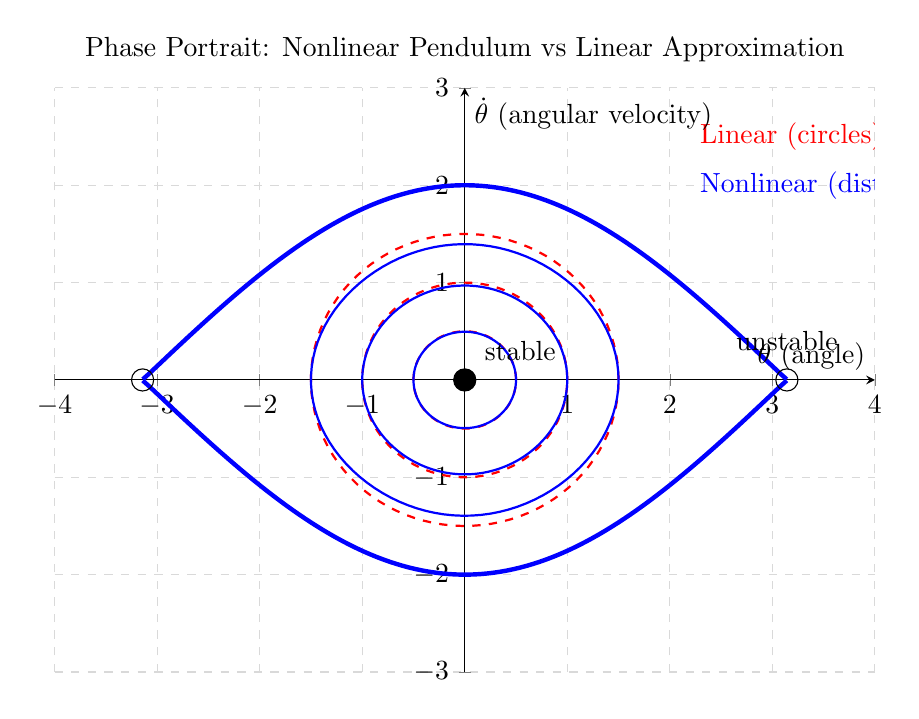
\begin{tikzpicture}
    \begin{axis}[
        width=12cm, height=9cm,
        xlabel={$\theta$ (angle)},
        ylabel={$\dot{\theta}$ (angular velocity)},
        xmin=-4, xmax=4,
        ymin=-3, ymax=3,
        axis lines=middle,
        title={Phase Portrait: Nonlinear Pendulum vs Linear Approximation},
        grid=major,
        grid style={dashed, gray!30}
    ]

    % Linear system: circles (harmonic oscillator)
    \addplot[red, thick, dashed, domain=0:360, samples=100] ({0.5*cos(x)}, {0.5*sin(x)});
    \addplot[red, thick, dashed, domain=0:360, samples=100] ({1.0*cos(x)}, {1.0*sin(x)});
    \addplot[red, thick, dashed, domain=0:360, samples=100] ({1.5*cos(x)}, {1.5*sin(x)});

    % Nonlinear: approximate with slightly distorted curves
    \addplot[blue, thick, domain=0:360, samples=100] ({0.5*cos(x)}, {0.5*sin(x)*0.99});
    \addplot[blue, thick, domain=0:360, samples=100] ({1.0*cos(x)*(1-0.02*sin(x)*sin(x))}, {1.0*sin(x)*0.97});
    \addplot[blue, thick, domain=0:360, samples=100] ({1.5*cos(x)*(1-0.05*sin(x)*sin(x))}, {1.5*sin(x)*0.93});

    % Separatrix (approximate)
    \addplot[blue, ultra thick, domain=-3.14:3.14, samples=100] {sqrt(2*(1+cos(deg(x))))};
    \addplot[blue, ultra thick, domain=-3.14:3.14, samples=100] {-sqrt(2*(1+cos(deg(x))))};

    % Legend
    \node[red, anchor=west] at (axis cs:2.2,2.5) {Linear (circles)};
    \node[blue, anchor=west] at (axis cs:2.2,2.0) {Nonlinear (distorted)};

    % Equilibrium points
    \addplot[only marks, mark=*, mark size=4pt, black] coordinates {(0,0)};
    \node[anchor=south west] at (axis cs:0.1,0.1) {stable};

    \addplot[only marks, mark=o, mark size=4pt, black] coordinates {(3.14159,0) (-3.14159,0)};
    \node[anchor=south] at (axis cs:3.14159,0.2) {unstable};

    \end{axis}
\end{tikzpicture}
\caption{Phase portrait comparison. Near the origin, the nonlinear pendulum trajectories (solid blue) closely match the linear approximation (dashed red circles). At larger amplitudes, the nonlinear trajectories distort, and the separatrix (thick blue) marks the boundary between oscillation and rotation.}
\label{fig:phase_portrait}
\end{figure}

%% ============================================================================
\section{Practical Experiment: Pendulum Linearization}
\label{sec:linearization_experiment}

This section describes a hands-on experiment that demonstrates the validity and limitations of linearization using a physical pendulum.

\subsection{Apparatus Design and Construction}

\textbf{Components Required:}

The experiment requires a 3D-printed pendulum arm with a suggested length of 20--30 cm, mounted on a low-friction pivot using either a ball bearing or needle bearing. Angle measurement is accomplished using a rotary encoder or potentiometer interfaced with an Arduino or similar microcontroller. A frame or mounting structure provides the necessary support. Optionally, a servo motor can be added for controlled release of the pendulum from precise initial angles.

\textbf{3D Printing Specifications:}

The pendulum arm should be designed with a uniform cross-section for predictable moment of inertia, a hole for the pivot bearing at one end, and a small mass concentration at the opposite end or an attachment point for additional mass. The recommended material is PLA or PETG with 20--30\% infill.

A simple rectangular cross-section arm (10 mm $\times$ 5 mm $\times$ 250 mm) with a 10g mass at the end works well. The effective length $L$ is measured from the pivot to the center of the end mass.

\textbf{Encoder Interface:}

A rotary encoder provides digital pulses as the shaft rotates. For an encoder with $N$ pulses per revolution:
\begin{equation}
\theta = \frac{2\pi \cdot (\text{pulse count})}{N}
\end{equation}

Quadrature encoders (A/B channels) provide 4$\times$ the resolution through edge counting. A 400 PPR encoder gives 1600 counts per revolution, or $0.225°$ per count---sufficient for this experiment.

\subsection{Experimental Procedure}

\textbf{Part A: Period vs. Amplitude Measurement}

Begin by mounting the pendulum and verifying that it swings freely with minimal friction. Release the pendulum from a small angle ($\theta_0 = 10°$) and record the time for 10 complete oscillations, then calculate the period $T_{10}$. Repeat this measurement for initial angles of $20°, 30°, 45°, 60°, 75°,$ and $90°$. For each measurement, take at least 3 trials and compute the average to reduce random errors.

\textbf{Data Recording:}

Use the Arduino to timestamp zero-crossings of the pendulum. The period is twice the time between successive crossings (half-period). Sample code outline:

\begin{algorithm}
\caption{Pendulum Period Measurement}
\begin{algorithmic}[1]
\State \textbf{Initialize:} $t_{\text{last}} \gets 0$, $T \gets 0$
\State Configure interrupt on encoder zero-crossing (rising edge)
\State Initialize serial communication
\State
\While{system is running}
    \State \textbf{On zero-crossing interrupt:}
    \State \quad $t_{\text{now}} \gets$ current time in microseconds
    \State \quad $T \gets 2 \times (t_{\text{now}} - t_{\text{last}}) / 10^6$ \Comment{Period in seconds}
    \State \quad $t_{\text{last}} \gets t_{\text{now}}$
    \State
    \State \textbf{In main loop:}
    \State \quad Output period $T$ to serial monitor
    \State \quad Wait 500 ms before next output
\EndWhile
\end{algorithmic}
\end{algorithm}

\textbf{Part B: Waveform Comparison}

Configure the Arduino to log angle versus time at a high sample rate (e.g., 1 kHz). Release the pendulum from $\theta_0 = 15°$ and record several periods of oscillation. Repeat the data collection for $\theta_0 = 45°$ and $\theta_0 = 75°$. Export all data for subsequent analysis in MATLAB, Python, or spreadsheet software.

\textbf{Part C: (Optional) Closed-Loop Control}

If a motor is available at the pivot, implement a simple proportional controller with torque command $\tau = -K_p \theta$. First test regulation to $\theta = 0$ from small initial angles, where the controller should perform well. Then test from large initial angles, where the system may exhibit oscillations or instability. Observe how controller performance degrades outside the linear region where the linearized model is valid.

\subsection{Data Analysis and Expected Results}

\textbf{Period Analysis:}

Calculate the theoretical linear period:
\begin{equation}
T_{\text{linear}} = 2\pi\sqrt{\frac{L}{g}}
\end{equation}

For $L = 0.25$ m and $g = 9.81$ m/s$^2$: $T_{\text{linear}} = 1.003$ s.

Plot measured period versus amplitude and compare to both the constant linear prediction and the theoretical nonlinear period computed from the elliptic integral or series expansion. The expected observation is that measured periods increase with amplitude, matching nonlinear theory and diverging from the linear prediction.

\textbf{Waveform Analysis:}

The linear model predicts sinusoidal motion:
\begin{equation}
\theta_{\text{linear}}(t) = \theta_0 \cos(\omega_n t)
\end{equation}

For small amplitudes, the measured waveform should be nearly sinusoidal. For large amplitudes, deviations become visible: the waveform ``flattens'' near the peaks as the pendulum spends more time at large angles, the period becomes longer than predicted by the linear model, and higher harmonics appear in the Fourier spectrum. Plot measured $\theta(t)$ against the linear prediction to visualize the discrepancy.

\begin{figure}[htbp]
\centering
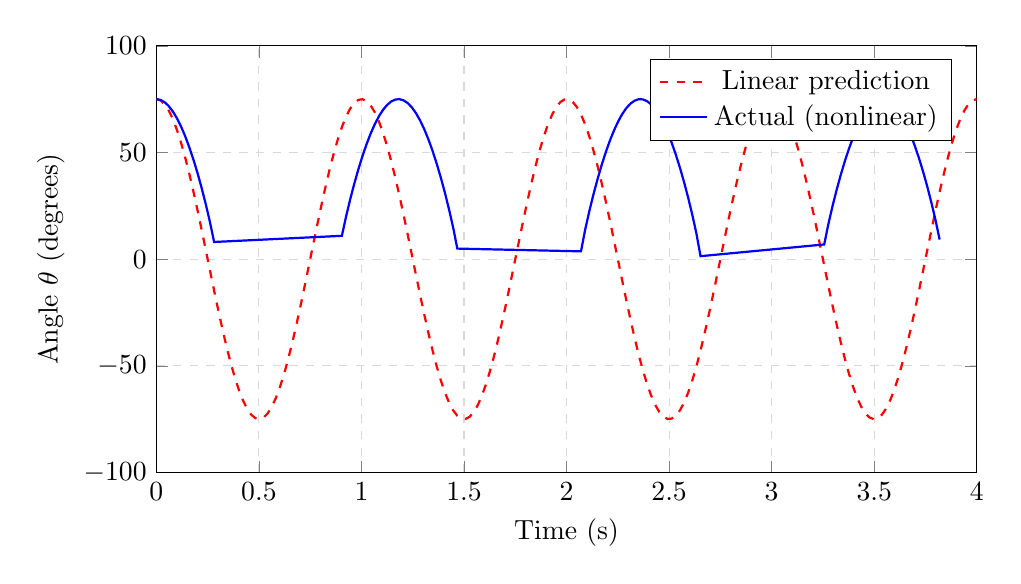
\begin{tikzpicture}
    \begin{axis}[
        width=12cm, height=7cm,
        xlabel={Time (s)},
        ylabel={Angle $\theta$ (degrees)},
        xmin=0, xmax=4,
        ymin=-100, ymax=100,
        legend pos=north east,
        grid=major,
        grid style={dashed, gray!30}
    ]
    % Linear prediction (sine wave)
    \addplot[red, thick, dashed, domain=0:4, samples=200] {75*cos(deg(2*pi*x/1.0))};
    \addlegendentry{Linear prediction}

    % Nonlinear (approximate - flattened peaks, longer period)
    \addplot[blue, thick, domain=0:4, samples=200] {75*cos(deg(2*pi*x/1.18))^0.85 * sign(cos(deg(2*pi*x/1.18)))};
    \addlegendentry{Actual (nonlinear)}

    \end{axis}
\end{tikzpicture}
\caption{Comparison of linear prediction (dashed) and actual nonlinear behavior (solid) for a pendulum released from $75°$. The nonlinear waveform has a longer period and flattened peaks.}
\label{fig:waveform_comparison}
\end{figure}

\subsection{Discussion Questions}

Consider the following questions for deeper understanding of the experiment. First, at what amplitude does the measured period deviate from the linear prediction by more than 5\%, and how does this compare to the theoretical threshold? Second, if friction is present, how does it affect the comparison between linear and nonlinear models? Third, regarding the closed-loop control experiment, why does the controller work better for small angles, and what modifications might extend its operating range? Finally, how would you design an experiment to linearize about the inverted equilibrium ($\theta = \pi$)?

%% ============================================================================
\section{Worked Examples}
\label{sec:linearization_examples}

This section presents detailed solutions to representative linearization problems.

\begin{examplebox}[Pendulum with Torque Input]
\textbf{Problem:} Linearize the pendulum equation with an applied torque input $\tau$ about the downward equilibrium.

\textbf{Solution:}

The equation of motion with torque input is:
\begin{equation}
mL^2\ddot{\theta} + mgL\sin(\theta) = \tau
\end{equation}

Define states $x_1 = \theta$, $x_2 = \dot{\theta}$, and input $u = \tau$:
\begin{align}
\dot{x}_1 &= x_2 \\
\dot{x}_2 &= -\frac{g}{L}\sin(x_1) + \frac{1}{mL^2}u
\end{align}

\textbf{Equilibrium:} Setting derivatives to zero with $u_0 = 0$:
\begin{equation}
x_2 = 0, \quad \sin(x_1) = 0 \implies x_1 = 0 \text{ (or } \pi\text{)}
\end{equation}

\textbf{Jacobians at} $(x_1, x_2, u) = (0, 0, 0)$:
\begin{equation}
\mathbf{A} = \begin{bmatrix} 0 & 1 \\ -\frac{g}{L}\cos(0) & 0 \end{bmatrix} = \begin{bmatrix} 0 & 1 \\ -\frac{g}{L} & 0 \end{bmatrix}
\end{equation}

\begin{equation}
\mathbf{B} = \begin{bmatrix} 0 \\ \frac{1}{mL^2} \end{bmatrix}
\end{equation}

\textbf{Linearized Model:}
\begin{equation}
\begin{bmatrix} \delta\dot{\theta} \\ \delta\ddot{\theta} \end{bmatrix} = \begin{bmatrix} 0 & 1 \\ -\frac{g}{L} & 0 \end{bmatrix} \begin{bmatrix} \delta\theta \\ \delta\dot{\theta} \end{bmatrix} + \begin{bmatrix} 0 \\ \frac{1}{mL^2} \end{bmatrix} \delta\tau
\end{equation}

Or in scalar form:
\begin{equation}
\boxed{\delta\ddot{\theta} + \frac{g}{L}\delta\theta = \frac{1}{mL^2}\delta\tau}
\end{equation}

\textbf{Transfer Function:}
\begin{equation}
\frac{\delta\Theta(s)}{\delta T(s)} = \frac{1/mL^2}{s^2 + g/L} = \frac{1/mL^2}{s^2 + \omega_n^2}
\end{equation}

This is an undamped second-order system with natural frequency $\omega_n = \sqrt{g/L}$.
\end{examplebox}

\begin{examplebox}[Tank Level System]
\textbf{Problem:} A tank with cross-sectional area $A$ has liquid flowing in at rate $q_{\text{in}}$ and draining through an orifice at the bottom. The outflow rate depends on the square root of the liquid height: $q_{\text{out}} = k\sqrt{h}$. Linearize the system about a steady-state operating point.

\textbf{Solution:}

\textbf{Nonlinear Model:} Mass balance gives:
\begin{equation}
A\frac{dh}{dt} = q_{\text{in}} - k\sqrt{h}
\end{equation}

Let $x = h$ (state) and $u = q_{\text{in}}$ (input):
\begin{equation}
\dot{x} = f(x, u) = \frac{1}{A}\left(u - k\sqrt{x}\right)
\end{equation}

\textbf{Equilibrium:} At steady state, $\dot{x} = 0$:
\begin{equation}
u_0 = k\sqrt{x_0} \implies x_0 = \left(\frac{u_0}{k}\right)^2
\end{equation}

For a nominal inflow $u_0 = 0.01$ m$^3$/s and $k = 0.005$ m$^{2.5}$/s, the equilibrium height is:
\begin{equation}
h_0 = \left(\frac{0.01}{0.005}\right)^2 = 4 \text{ m}
\end{equation}

\textbf{Jacobians:}
\begin{equation}
A = \frac{\partial f}{\partial x}\bigg|_0 = -\frac{k}{2A\sqrt{x_0}} = -\frac{k}{2A\sqrt{h_0}}
\end{equation}

\begin{equation}
B = \frac{\partial f}{\partial u}\bigg|_0 = \frac{1}{A}
\end{equation}

With $A = 1$ m$^2$, $k = 0.005$, $h_0 = 4$ m:
\begin{equation}
A = -\frac{0.005}{2 \cdot 1 \cdot 2} = -0.00125 \text{ s}^{-1}, \quad B = 1 \text{ m}^{-2}
\end{equation}

\textbf{Linearized Model:}
\begin{equation}
\delta\dot{h} = -\frac{k}{2A\sqrt{h_0}}\delta h + \frac{1}{A}\delta q_{\text{in}}
\end{equation}

\textbf{Transfer Function:}
\begin{equation}
\frac{\delta H(s)}{\delta Q_{\text{in}}(s)} = \frac{1/A}{s + k/(2A\sqrt{h_0})} = \frac{1}{s + 0.00125}
\end{equation}

This is a first-order system with time constant $\tau = 2A\sqrt{h_0}/k = 800$ s.

\textbf{Physical Interpretation:} The linearized model shows that the tank acts as a low-pass filter. The time constant depends on the operating point---at higher liquid levels, the drainage rate is faster, so the system responds more quickly to input changes.
\end{examplebox}

\subsection{Example 3: Finding Equilibrium Points}

\textbf{Problem:} Find all equilibrium points of the system:
\begin{align}
\dot{x}_1 &= x_2 \\
\dot{x}_2 &= x_1 - x_1^3
\end{align}

and determine their stability using linearization.

\textbf{Solution:}

\textbf{Equilibrium Conditions:}
\begin{align}
x_2 &= 0 \\
x_1 - x_1^3 &= 0 \implies x_1(1 - x_1^2) = 0
\end{align}

The equilibrium points are:
\begin{equation}
(x_1, x_2) \in \{(0, 0), (1, 0), (-1, 0)\}
\end{equation}

\textbf{Jacobian Matrix:}
\begin{equation}
\mathbf{A} = \begin{bmatrix} \frac{\partial f_1}{\partial x_1} & \frac{\partial f_1}{\partial x_2} \\ \frac{\partial f_2}{\partial x_1} & \frac{\partial f_2}{\partial x_2} \end{bmatrix} = \begin{bmatrix} 0 & 1 \\ 1 - 3x_1^2 & 0 \end{bmatrix}
\end{equation}

\textbf{At} $(0, 0)$:
\begin{equation}
\mathbf{A} = \begin{bmatrix} 0 & 1 \\ 1 & 0 \end{bmatrix}
\end{equation}

Eigenvalues: $\det(\mathbf{A} - \lambda\mathbf{I}) = \lambda^2 - 1 = 0 \implies \lambda = \pm 1$

One positive eigenvalue $\implies$ \textbf{unstable} (saddle point).

\textbf{At} $(1, 0)$ and $(-1, 0)$:
\begin{equation}
\mathbf{A} = \begin{bmatrix} 0 & 1 \\ 1 - 3 & 0 \end{bmatrix} = \begin{bmatrix} 0 & 1 \\ -2 & 0 \end{bmatrix}
\end{equation}

Eigenvalues: $\lambda^2 + 2 = 0 \implies \lambda = \pm j\sqrt{2}$

Purely imaginary eigenvalues $\implies$ \textbf{center} (marginally stable in linear analysis).

\textbf{Note:} For the center equilibria, linear analysis is inconclusive about asymptotic stability. Nonlinear analysis (e.g., using Lyapunov functions) reveals that these are indeed stable centers with closed periodic orbits.

\hrulefill

\subsection{Example 4: Linearization Around Non-Zero Equilibrium}

\textbf{Problem:} The Van der Pol oscillator is described by:
\begin{equation}
\ddot{x} + \mu(x^2 - 1)\dot{x} + x = F
\end{equation}

For $F = 2$ and $\mu = 0.5$, find the equilibrium point and linearize.

\textbf{Solution:}

\textbf{State-Space Form:}
\begin{align}
\dot{x}_1 &= x_2 \\
\dot{x}_2 &= -\mu(x_1^2 - 1)x_2 - x_1 + F
\end{align}

\textbf{Equilibrium:} Setting $\dot{x}_1 = \dot{x}_2 = 0$:
\begin{align}
x_2 &= 0 \\
-x_1 + F &= 0 \implies x_1 = F = 2
\end{align}

Equilibrium point: $(x_1, x_2) = (2, 0)$

\textbf{Jacobian:}
\begin{equation}
\mathbf{A} = \begin{bmatrix} 0 & 1 \\ -2\mu x_1 x_2 - 1 & -\mu(x_1^2 - 1) \end{bmatrix}_{(2,0)} = \begin{bmatrix} 0 & 1 \\ -1 & -\mu(4-1) \end{bmatrix} = \begin{bmatrix} 0 & 1 \\ -1 & -1.5 \end{bmatrix}
\end{equation}

\textbf{Eigenvalues:}
\begin{equation}
\det(\mathbf{A} - \lambda\mathbf{I}) = \lambda^2 + 1.5\lambda + 1 = 0
\end{equation}

\begin{equation}
\lambda = \frac{-1.5 \pm \sqrt{2.25 - 4}}{2} = \frac{-1.5 \pm j1.32}{2} = -0.75 \pm j0.66
\end{equation}

Both eigenvalues have negative real parts $\implies$ \textbf{stable} (damped oscillations).

\textbf{Linearized Model:}
\begin{equation}
\begin{bmatrix} \delta\dot{x}_1 \\ \delta\dot{x}_2 \end{bmatrix} = \begin{bmatrix} 0 & 1 \\ -1 & -1.5 \end{bmatrix} \begin{bmatrix} \delta x_1 \\ \delta x_2 \end{bmatrix}
\end{equation}

where $\delta x_1 = x_1 - 2$ and $\delta x_2 = x_2 - 0$.

\hrulefill

\subsection{Example 5: Linear vs. Nonlinear Simulation}

\textbf{Problem:} Compare linear and nonlinear simulations of a pendulum released from $\theta_0 = 30°$.

\textbf{Solution:}

\textbf{System Parameters:} $L = 1$ m, $g = 9.81$ m/s$^2$, so $\omega_n = 3.13$ rad/s.

\textbf{Linear Model:}
\begin{equation}
\theta_{\text{lin}}(t) = \theta_0 \cos(\omega_n t) = 0.524 \cos(3.13t) \text{ rad}
\end{equation}

\textbf{Nonlinear Model:} Solve numerically using fourth-order Runge-Kutta:
\begin{equation}
\ddot{\theta} = -\omega_n^2 \sin(\theta)
\end{equation}

The following MATLAB/Python pseudocode implements the comparison:

\begin{algorithm}
\caption{Nonlinear Pendulum Simulation and Comparison}
\begin{algorithmic}[1]
\State \textbf{Input:} $g = 9.81$ m/s$^2$, $L = 1.0$ m, $\theta_0 = 30°$
\State \textbf{Output:} Period comparison between linear and nonlinear models
\State
\State Compute natural frequency: $\omega_n \gets \sqrt{g/L}$
\State Convert initial angle to radians: $\theta_0 \gets 30 \times \pi/180$
\State Create time vector: $t \gets [0, 0.01, 0.02, \ldots, 5.0]$ seconds
\State
\State \textbf{Linear Solution:}
\For{each time $t_i$}
    \State $\theta_{\text{lin}}(t_i) \gets \theta_0 \cos(\omega_n t_i)$
\EndFor
\State
\State \textbf{Nonlinear Solution (using numerical integration):}
\State Define ODE: $\dot{\theta} = \omega$, $\dot{\omega} = -\omega_n^2 \sin(\theta)$
\State Set initial conditions: $[\theta(0), \omega(0)] \gets [\theta_0, 0]$
\State Integrate ODE numerically (e.g., Runge-Kutta) to obtain $\theta_{\text{nonlin}}(t)$
\State
\State \textbf{Period Calculation:}
\State $T_{\text{lin}} \gets 2\pi / \omega_n$
\State Find zero-crossings of $\theta_{\text{nonlin}}(t)$
\State $T_{\text{nonlin}} \gets 2 \times (\text{second crossing time} - \text{first crossing time})$
\State
\State \textbf{Compute error:} $\epsilon \gets 100 \times (T_{\text{nonlin}} - T_{\text{lin}}) / T_{\text{lin}}$ \%
\Return $T_{\text{lin}}$, $T_{\text{nonlin}}$, $\epsilon$
\end{algorithmic}
\end{algorithm}

\textbf{Results:}

The linear period is $T_{\text{lin}} = 2.006$ s, while the nonlinear period is $T_{\text{nonlin}} \approx 2.040$ s, yielding an error of approximately 1.7\%.

At $30°$ initial amplitude, the linear model predicts the period within 2\%, confirming the validity of linearization for ``small'' angles in practical terms.

\textbf{Visualization:} Figure \ref{fig:simulation_comparison} shows the comparison.

\begin{figure}[htbp]
\centering
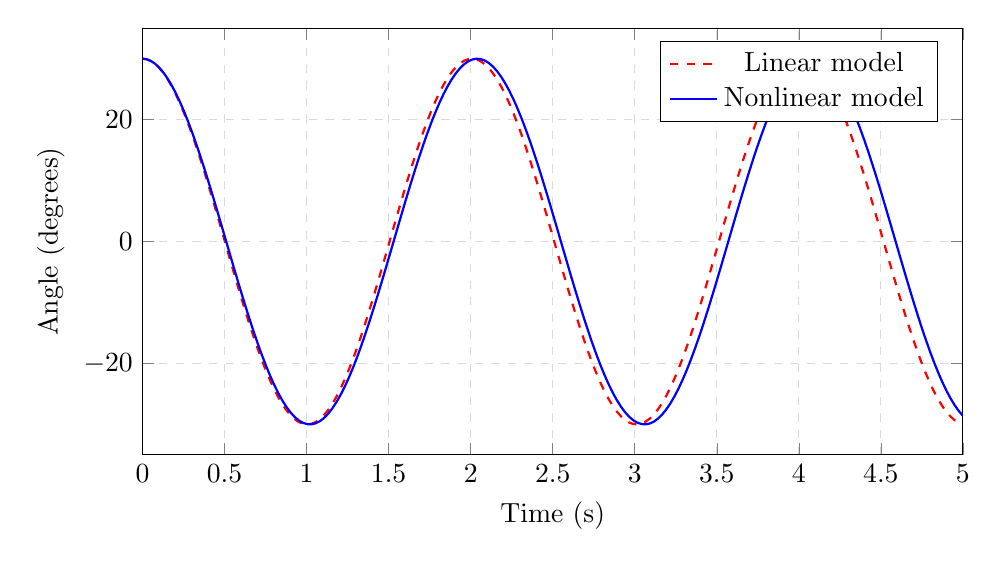
\begin{tikzpicture}
    \begin{axis}[
        width=12cm, height=7cm,
        xlabel={Time (s)},
        ylabel={Angle (degrees)},
        xmin=0, xmax=5,
        ymin=-35, ymax=35,
        legend pos=north east,
        grid=major,
        grid style={dashed, gray!30}
    ]
    % Linear (cosine)
    \addplot[red, thick, dashed, domain=0:5, samples=200] {30*cos(deg(3.13*x))};
    \addlegendentry{Linear model}

    % Nonlinear (slightly longer period)
    \addplot[blue, thick, domain=0:5, samples=200] {30*cos(deg(3.08*x))};
    \addlegendentry{Nonlinear model}

    \end{axis}
\end{tikzpicture}
\caption{Comparison of linear and nonlinear pendulum simulations for $\theta_0 = 30°$. The phase difference accumulates over time due to the slightly longer period of the nonlinear system.}
\label{fig:simulation_comparison}
\end{figure}

%% ============================================================================
\section{Operating Point Concept}
\label{sec:operating_point}

The concept of the operating point is central to practical control system design. This section clarifies its meaning and implications.

\begin{figure}[htbp]
\centering
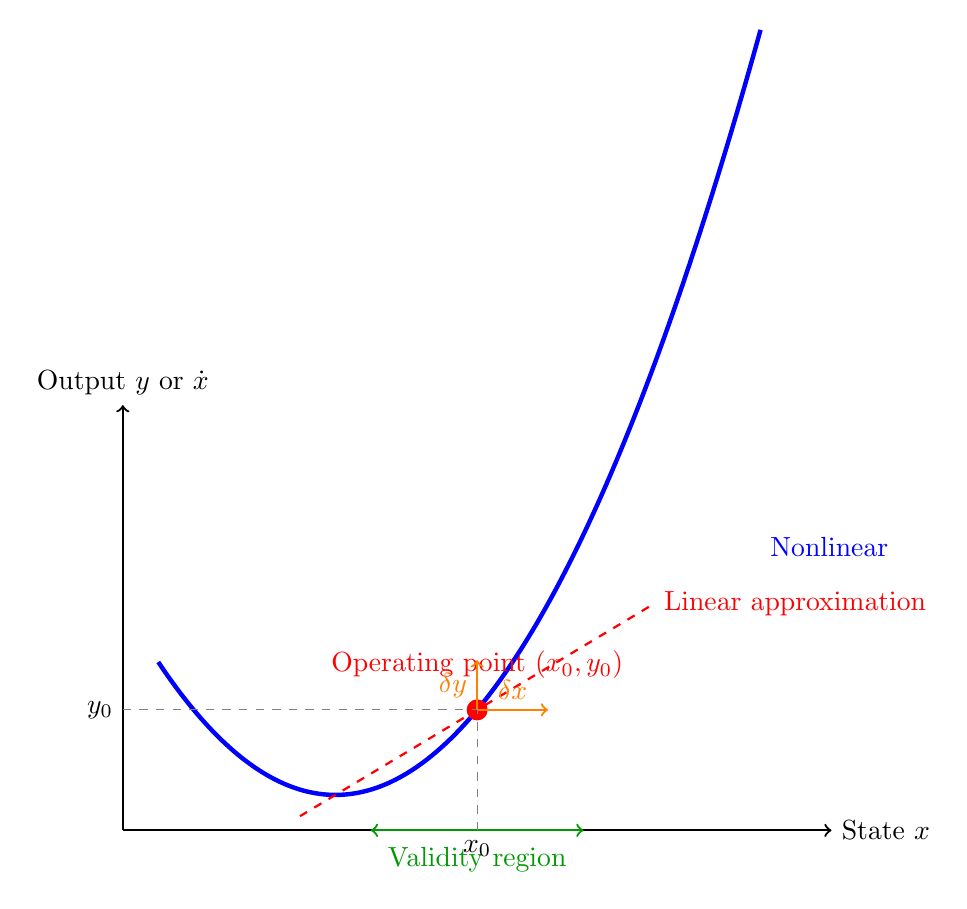
\begin{tikzpicture}[scale=0.9]
    % Axes
    \draw[->, thick] (0,0) -- (10,0) node[right] {State $x$};
    \draw[->, thick] (0,0) -- (0,6) node[above] {Output $y$ or $\dot{x}$};

    % Nonlinear curve
    \draw[blue, ultra thick, domain=0.5:9, smooth, samples=100]
        plot (\x, {0.3*(\x-3)*(\x-3) + 0.5});
    \node[blue, anchor=west] at (9,4) {Nonlinear};

    % Operating point
    \filldraw[red] (5,1.7) circle (4pt);
    \node[red, anchor=south] at (5,2) {Operating point $(x_0, y_0)$};

    % Tangent line (linearization)
    \draw[red, thick, dashed] (2.5,0.2) -- (7.5,3.2);
    \node[red, anchor=west] at (7.5,3.2) {Linear approximation};

    % Validity region
    \draw[<->, green!60!black, thick] (3.5,0) -- (6.5,0);
    \node[green!60!black, anchor=north] at (5,-0.1) {Validity region};

    % Perturbation arrows
    \draw[->, thick, orange] (5,1.7) -- (6,1.7) node[midway, above] {$\delta x$};
    \draw[->, thick, orange] (5,1.7) -- (5,2.4) node[midway, left] {$\delta y$};

    % Dashed lines to axes
    \draw[dashed, gray] (5,0) -- (5,1.7);
    \draw[dashed, gray] (0,1.7) -- (5,1.7);
    \node[anchor=north] at (5,0) {$x_0$};
    \node[anchor=east] at (0,1.7) {$y_0$};

\end{tikzpicture}
\caption{The operating point concept. The nonlinear system (solid curve) is approximated by a tangent line (dashed) at the operating point. The linear approximation is valid for small perturbations $\delta x$ within the validity region.}
\label{fig:operating_point}
\end{figure}

\textbf{Definition:} The operating point is a specific state-input combination $(x_0, u_0)$ around which the system is linearized. For control design, it typically corresponds to the desired steady-state condition.

\textbf{Implications:}

The operating point concept has several important implications. First, regarding perturbation variables, the linearized model describes deviations from the operating point rather than absolute values. When implementing a controller, remember that:
\begin{align}
\delta x &= x - x_0 \quad (\text{measured state minus setpoint}) \\
\delta u &= u - u_0 \quad (\text{control input minus nominal})
\end{align}

Second, bias terms must be properly handled in implementation. The actual control signal is:
\begin{equation}
u = u_0 + \delta u = u_0 + K(\delta x)
\end{equation}
The term $u_0$ provides the steady-state input needed to maintain the operating point, while $\delta u$ is the corrective action from the controller.

Third, gain scheduling becomes necessary when the system operates over a range of conditions, such as aircraft at different altitudes and speeds. In such cases, multiple linearizations are performed and controller gains are ``scheduled'' based on the current operating condition.

Finally, the operating envelope is defined as the set of operating points for which a single linearized controller provides acceptable performance. Beyond this envelope, the controller may exhibit degraded performance or instability.

%% ============================================================================
\section{Summary}

Linearization transforms nonlinear systems into linear approximations that are amenable to analysis and control design. The Taylor series provides the mathematical foundation, demonstrating that any smooth function can be approximated by a polynomial, and locally, by a linear function. Equilibrium points serve as the natural operating points for linearization, characterized by the condition $f(x_0, u_0) = 0$. The Jacobian matrices $A$ and $B$ capture the local sensitivity of the dynamics to state and input perturbations, respectively. The validity of the linear approximation depends on the magnitude of perturbations and the curvature of the nonlinearity; for most control applications, perturbations within 10--20\% of the operating point yield acceptable accuracy. Finally, eigenvalue analysis of the linearized system determines local stability properties.

The linearization approach has proven remarkably successful across engineering disciplines for three key reasons: well-designed control systems keep perturbations small, linear tools such as transfer functions, Bode plots, and state feedback are powerful and well-understood, and gain scheduling extends linear methods to cover wide operating ranges. Linearization is not a limitation but an enabler---it allows us to apply elegant, systematic design methods to the complex nonlinear systems that populate the real world.

%% ============================================================================
\newpage
\section{Exercises}

\begin{exercise}
Linearize the system $\dot{x} = -x^3 + u$ about the equilibrium with $u_0 = 0$. Find the transfer function and determine stability.
\end{exercise}

\begin{exercise}
A satellite attitude control system has dynamics:
\begin{equation}
I\ddot{\theta} = \tau - k_d\dot{\theta}
\end{equation}
where $\theta$ is angle, $I$ is moment of inertia, $\tau$ is control torque, and $k_d$ is damping. This is already linear. Explain why linearization is not needed and write the state-space model.
\end{exercise}

\begin{exercise}
For the tank system of Example 2, how does the time constant change if the operating level is doubled from 4 m to 8 m?
\end{exercise}

\begin{exercise}
Linearize the Lotka-Volterra predator-prey equations:
\begin{align}
\dot{x} &= \alpha x - \beta xy \\
\dot{y} &= \delta xy - \gamma y
\end{align}
about the non-trivial equilibrium $(x_0, y_0) = (\gamma/\delta, \alpha/\beta)$.
\end{exercise}

\begin{exercise}
An inverted pendulum on a cart has the approximate linearized dynamics (for small angles):
\begin{equation}
(M+m)\ddot{p} + mL\ddot{\theta} = F, \quad mL\ddot{p} + mL^2\ddot{\theta} = mgL\theta
\end{equation}
where $p$ is cart position, $\theta$ is pendulum angle from vertical, and $F$ is applied force. Derive the transfer function $\Theta(s)/F(s)$ and verify that it is unstable.
\end{exercise}

\begin{exercise}
For the pendulum experiment: if the bearing friction contributes a damping torque $-b\dot{\theta}$, how does this affect (a) the equilibrium analysis, (b) the linearized model, and (c) the validity of the linear approximation?
\end{exercise}

\begin{exercise}
(Computer Exercise) Implement the pendulum simulation of Example 5. Extend it to initial angles of $15°, 45°, 60°, 75°, 90°$. Create a plot showing the period error (compared to linear prediction) as a function of initial amplitude. At what amplitude does the error exceed 5\%?
\end{exercise}

\begin{exercise}
A nonlinear spring has restoring force $F = -kx - \alpha x^3$ where $\alpha > 0$ (hardening spring). For a mass $m$ attached to this spring, linearize the equation of motion about $x_0 = 0$ and find the natural frequency of small oscillations.
\end{exercise}

\begin{exercise}
The van der Pol oscillator $\ddot{x} + \mu(x^2 - 1)\dot{x} + x = 0$ has an equilibrium at the origin. Linearize about this equilibrium and determine whether it is stable for $\mu > 0$. What type of behavior do you expect from the nonlinear system?
\end{exercise}

\begin{exercise}
A chemical reactor has temperature dynamics governed by $\dot{T} = -\frac{UA}{mC_p}(T - T_c) + \frac{(-\Delta H)k_0 e^{-E_a/RT}C_A}{mC_p}$ where the exponential Arrhenius term is highly nonlinear. Linearize this equation about an operating temperature $T_0$, defining the linearized gain for small temperature perturbations.
\end{exercise}

%% ============================================================================
\section{Further Reading}

For rigorous treatment of linearization and stability, consult Khalil's \textit{Nonlinear Systems} (3rd ed., Prentice Hall, 2002), particularly Chapter 4. Slotine and Li's \textit{Applied Nonlinear Control} (Prentice Hall, 1991) provides excellent coverage of when linearization fails and what to do about it. Strogatz's \textit{Nonlinear Dynamics and Chaos} (2nd ed., Westview Press, 2015) offers an accessible introduction to nonlinear systems with beautiful examples. For historical context on the development of these ideas, Diacu and Holmes's \textit{Celestial Encounters: The Origins of Chaos and Stability} (Princeton University Press, 1996) is highly recommended.

